\chapter{Using JAGS}
JAGS stands for ``Just Another Gibbs Sampler''. JAGS is a computer program that
allows the user
to implement Markov Chain Monte Carlo (MCMC) on fairly complicated problems
very quickly. The ``Gibbs Sampling'' mentioned in the name of JAGS
is a particular MCMC technique that is beyond the
scope of this course: however, it is not so different from the Metropolis-Hastings
method that we do study in this course. If you are faced with a statistics
problem which you would like to solve in a Bayesian way, JAGS makes it very
straightforward to implement a Bayesian model. Essentially, you just need to tell
JAGS the following things:
\begin{itemize}
\item The names of your unknown parameter(s), and their prior distributions
\item The likelihood
\end{itemize}
Then we simply load in the data and let it go! JAGS will run MCMC, automatically
choosing an appropriate starting point based on your prior,
and moving the parameter
values around so the posterior distribution is well sampled.
In this chapter we will see how to use JAGS with a simple example, and we will
see some more features of JAGS when we come to study more complex examples.
There are some more advanced features of JAGS that we will not use in this
course.

JAGS is not the first program of its kind, and it is related to many other
available programs.
Starting in the late 1980s, a program called BUGS (Bayesian inference Using
Gibbs Sampling) was developed, and this evolved into the program WinBUGS. These
programs had a huge effect on the uptake of Bayesian statistics, by dramatically
reducing the amount of work it takes to get an MCMC simulation to run. Instead
of having to code up your own implementation of the Metropolis algorithm or
an alternative MCMC method, all you had to do was tell WinBUGS what your prior
and likelihood were, and it would automatically use appropriate and sophisticated
MCMC methods.

Up until 2012, STATS 331 was taught using WinBUGS.
However, there are a number of disadvantages to
WinBUGS, so I decided to switch over to JAGS in 2013. The main advantages of
JAGS over WinBUGS are: i) it is open source software and works on all
operating systems, ii) it allows a more concise version of notation that can
save a lot of space and make the code easier to read and write, and iii) 
WinBUGS is not actively developed or maintained any more. In addition, a lot of time in previous iterations of 331 was spent teaching
different ways of using WinBUGS (i.e. calling it from R, vs. using the graphical
interface, vs. writing a script). In 2013 we will use JAGS in just one way (by calling it from R), which frees up time for us to concentrate on the stats!
There is another up to date BUGS program called OpenBUGS, but it too is only
a Windows program. Most of what you learn about JAGS can be transferred to
WinBUGS or OpenBUGS quite easily, if necessary, with only minor changes.

\section{Basic JAGS Example}
Since we have used it a lot already, it makes sense to look at how the bus
problem looks in JAGS. Recall we had a
single unknown parameter $\theta$, with a uniform prior between 0 and 1.
We also had a binomial likelihood, which we could write as
$x \sim \textnormal{Binomial}(N, \theta)$.
To implement this model in JAGS, the code looks like this:
\begin{framed}
\begin{verbatim}
model
{
    # Parameters and the priors
    theta ~ dunif(0, 1)

    # Likelihood
    x ~ dbin(theta, N)
}
\end{verbatim}
\end{framed}
As in R, comments (statements that have no effect but help to annotate the
code) can be written with a \# symbol.
The names of the distributions in JAGS are very similar to (but not always
exactly the same as) the names of the R functions for evaluating the probability
densities or mass functions. In this example, {\tt dunif} is the uniform
distribution and {\tt dbin} is the binomial distribution. One final thing to
note is the order of the parameters in the binomial distribution. In JAGS the
success probability comes first and the number of trials comes second.
There are some quirks with the other distributions as well, such as the normal
distribution, which we will see in later chapters.

The code for implementing a Bayesian model in JAGS belongs inside
a {\tt model\{   \}} block.
In our example,
the first statement inside the model is {\tt theta \~{ } dunif(0, 1)}. As you
can probably guess, {\tt theta}
is simply the name of our parameter. We are free to name it as we
wish, and in different situations we will give the parameters different names.
The tilde sign is like the ``$\sim$'' notation for probability distributions.
We are
about to specify a probability distribution that applies to {\tt theta}. Finally,
the actual distribution is given, which is a uniform distribution between 0 and 1. Note
the command used for a uniform distribution is {\tt dunif} and not {\tt uniform}.
{\it Our line of code {\tt theta \~{ } dunif(0, 1)}
tells JAGS
there is a parameter called {\tt theta} and we want to use a uniform prior between
0 and 1}.

The notation for the likelihood is very similar. We write the name of the data
followed by ``{\tt \~{ }}'' and then the distribution, in this case the
binomial distribution.
One annoying this about the binomial distribution is the ordering of the parameters.
Usually people write the number of trials first and the success probability
second, but in JAGS it's the other way around.

Interestingly, the likelihood part of the code looks exactly like the
prior part. So how does JAGS know that {\tt x} is data and not just another
parameter? Well, when we call JAGS from R, we will pass to it an R list containing
the data. There will be a value for {\tt x} in this list, which tells JAGS that
it is a fixed and known quantity, and not another unknown parameter like {\tt theta}.

Above, we specified the JAGS model, but this isn't the only thing we need.
We also need a way to actually run JAGS! The most
convenient way to use JAGS is to call it from R, using the R library
{\tt rjags}. This way, the output (samples from the posterior distribution for
the parameters) is available in R for postprocessing such as plots and
smmaries. The
{\tt rjags} library has many features and options, and it can be a bit
overwhelming to figure out all of them using the documentation.
Therefore, I have written a template
R script called {\tt use\_jags.r} where you can specify the data, the JAGS
model, and some options at the
top of the file, and you do not have to worry about all the functions for
calling JAGS from R.

The first part of {\tt use\_jags.r} is given below. This is the part you
can modify to load different data, change the model assumptions, and decide
how long (for how many iterations or steps) you would like the MCMC to run for.

The {\it burn-in} is an initial part of the
MCMC run where results are not saved. This is beneficial because sometimes
it can take a while for the MCMC to locate the regions of high posterior
probability, and if you include the initial parts of the run in you results,
you can get incorrect answers. For most of our models in STATS 331, we do not
need a long burn-in period.

\begin{framed}
\begin{verbatim}
model = "model
{
  theta ~ dunif(0, 1)
  x ~ dbin(theta, N)
}
"

# The data (use NA for no data)
data = list(x=2, N=5)

# Variables to monitor
variable_names = c('theta')

# How many burn-in steps?
burn_in = 1000

# How many proper steps?
steps = 10000

# Thinning?
thin = 1
\end{verbatim}
\end{framed}

The second part of {\tt use\_jags.r} actually runs JAGS. You won't need to edit
this or know much about it, but for completeness, here it is:

\begin{framed}
\begin{verbatim}
# NO NEED TO EDIT PAST HERE!!!
# Just run it all and use the results list.

library('rjags')

# Write model out to file
fileConn=file("model.temp")
writeLines(model, fileConn)
close(fileConn)

if(all(is.na(data)))
{
    m = jags.model(file="model.temp")
} else
{
    m = jags.model(file="model.temp", data=data)
}
update(m, burn_in)
draw = jags.samples(m, steps, thin=thin, variable.names = variable_names)
# Convert to a list
make_list <- function(draw)
{
  results = list()
  for(name in names(draw))
  {
    # Extract "chain 1"
    results[[name]] = as.array(draw[[name]][,,1])
    
    # Transpose 2D arrays
    if(length(dim(results[[name]])) == 2)
      results[[name]] = t(results[[name]])
  }
  return(results)
}
results = make_list(draw)
\end{verbatim}
\end{framed}

When this code is executed, it creates an R list called {\tt results}.
Inside {\tt results}, there is a vector
for each variable that you chose to ``monitor'' by listing its name in
the {\tt variable\_names} vector. In this example there is only one parameter,
so it seems obvious we would like to monitor it. In more complex situations there
may be many parameters, and only some of them are actually interesting, the others
are ``nuisance parameters''. The {\tt variable\_names} vector allows you to choose
just the parameters you really care about.
Notice also the various options such as the number of steps, and the {\tt thin}
option. If {\tt thin} is set to 10, for example, only every 10th iteration
of the MCMC will appear in the results. This is useful for keeping the size
of the {\tt results} list manageable, even if you run the MCMC for a very
long time.

One of the most important things to check after running JAGS is a {\it trace
plot} of the parameters. A trace plot is a plot of the value of the parameter
over time, as the MCMC was running.
To plot a trace plot of the MCMC run, we can simply use the following code,
for a parameter called {\tt theta}. If the parameter has a different name,
replace {\tt theta} with the actual name of the parameter.
\begin{framed}
\begin{verbatim}
plot(results$theta, type='l')
\end{verbatim}
\end{framed}

You could look at the posterior distribution using a
histogram, and you can compute summaries using the methods discussed in
Chapter~\ref{chapter:summaries}. The code for the histogram for a parameter
{\tt theta} is given below.

\begin{framed}
\begin{verbatim}
hist(results$theta, breaks=100)
\end{verbatim}
\end{framed}

Examples of a trace plot and a histogram are given in Figure~\ref{fig:results}.
Trace plots are the best diagnostic tool for seeing whether MCMC is working
properly. Ideally, trace plots should look like ``noise'', without strong
correlations
between one point and the next. If there are strong correlations in the
trace plot, the MCMC will need to be run for a longer period of time to obtain
effectively independent samples from the posterior distribution.

\begin{figure}[ht!]
\begin{center}
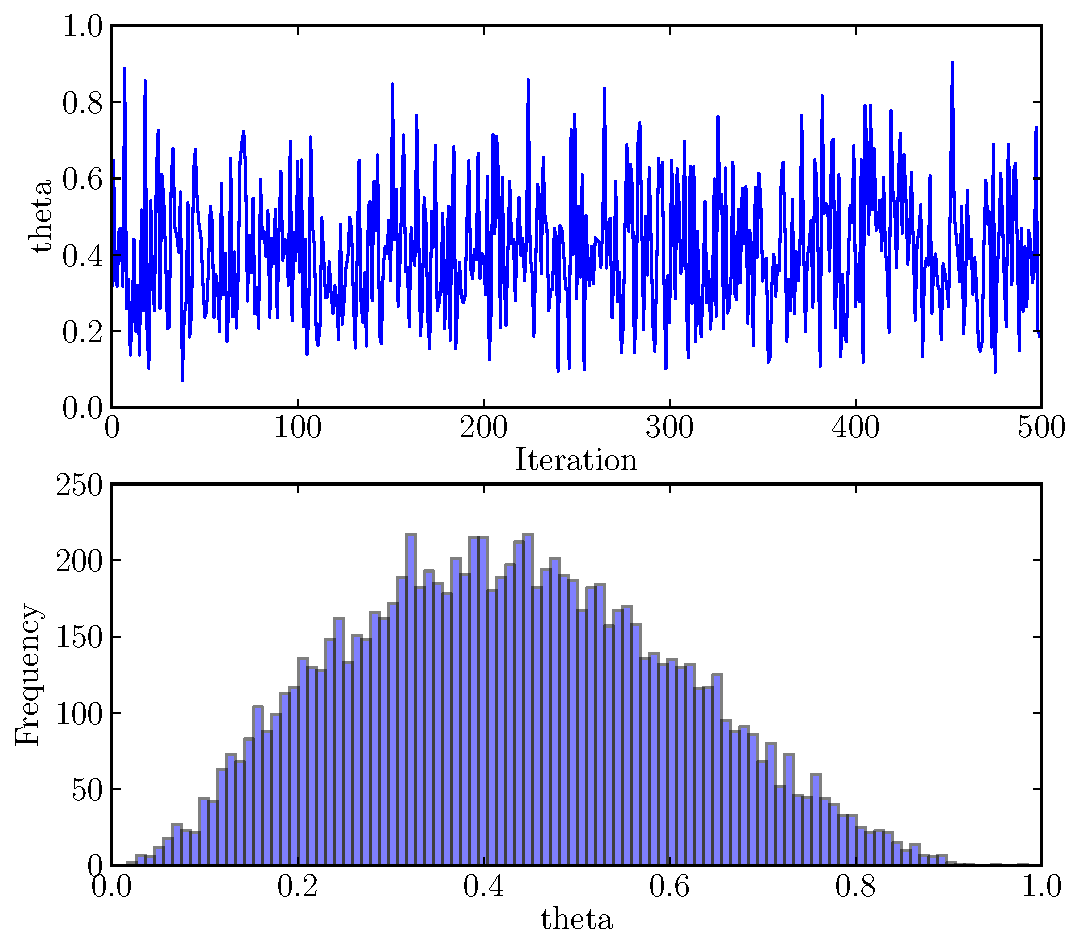
\includegraphics[scale=0.5]{Figures/jags_example.pdf}
\caption{\it The trace plot and histogram of the MCMC samples returned by
JAGS. The trace plot (top) is zoomed in on the first 500 samples, and shows the
{\tt theta} value moving around as the MCMC proceeds. The histogram of {\tt
theta} values, sampled from the posterior distribution, is given in the lower
panel. You can compare this with Figure~\ref{fig:bus_inference}.
\label{fig:results}}
\end{center}
\end{figure}

\section{Checklist for Using JAGS}
When running JAGS using the {\tt use\_jags.r} script provided, there are several
things you need to ensure. These are listed below.

\begin{itemize}
\item The data you want to analyse must be contained in an R
list called {\tt data}. Inside this list you should also include variables
such as the size of the data set (which I usually call {\tt N}),
or any other known constants that are
referred to in the model.
\item The JAGS model must be correctly written inside the R string called
{\tt model}. In the likelihood part of the JAGS model, you must ensure that
the names of the data variables match the names in your {\tt data} list. In
the example of this chapter, the number of successes is called {\tt x} in both
the data list and in the JAGS model.
\item The {\tt variable\_names} vector, which lists the parameters you are
interested in, can only list parameters that actually exist in the JAGS model.
If you try to monitor a variable that isn't in your model, you will get an
error message.
\end{itemize}
